\documentclass[a4paper,12pt]{article}

\usepackage{epsf,psfrag,graphicx}
\usepackage{hyperref,amssymb}
\usepackage{verbatim}

\newcommand{\qchem}{\href{http://q-chem.com}{{\scshape Q-Chem}}}
\newcommand{\iqmol}{\href{http://iqmol.org}{{\scshape IQmol}}}

\newcommand{\heading}[1]{ \noindent{ \large \bf{#1} }}
\newcommand{\myline}{\setlength{\unitlength}{1mm}
                     \begin{picture}(160,2)
                     \put(0,0){\line(1,0){160}}
                     \put(0,1){\line(1,0){160}}
                     \end{picture}
                    }
\newcommand{\showlines}[1]{}

\newcommand{\alert}[1]{\textcolor{red}{#1}}
\newcommand{\sci}[2]{\ensuremath{#1\times 10^{-#2}}}
\newcommand{\mc}{\multicolumn}
\newcommand{\R}[1]{\ensuremath{\mathrm{#1}}}
\newcommand{\B}[1]{\ensuremath{\mathbf{#1}}}



\setlength{\headheight}{0cm}
\setlength{\headsep}{0cm}
\setlength{\voffset}{0cm}
\setlength{\topmargin}{-0.3cm}
\setlength{\oddsidemargin}{0cm}
\setlength{\evensidemargin}{0cm}
\setlength{\hoffset}{0cm}
\setlength{\textheight}{25.0cm}
\setlength{\textwidth}{16cm}

\setlength{\parindent}{0cm}
\setlength{\unitlength}{1mm}

\pagestyle{empty}

%----------------------------------------------------------------------%
\begin{document}
%----------------------------------------------------------------------%

\noindent
\myline\\
\begin{center}
{\LARGE Introduction to IQmol}
\end{center}
\myline\\

\vfill

\begin{center}
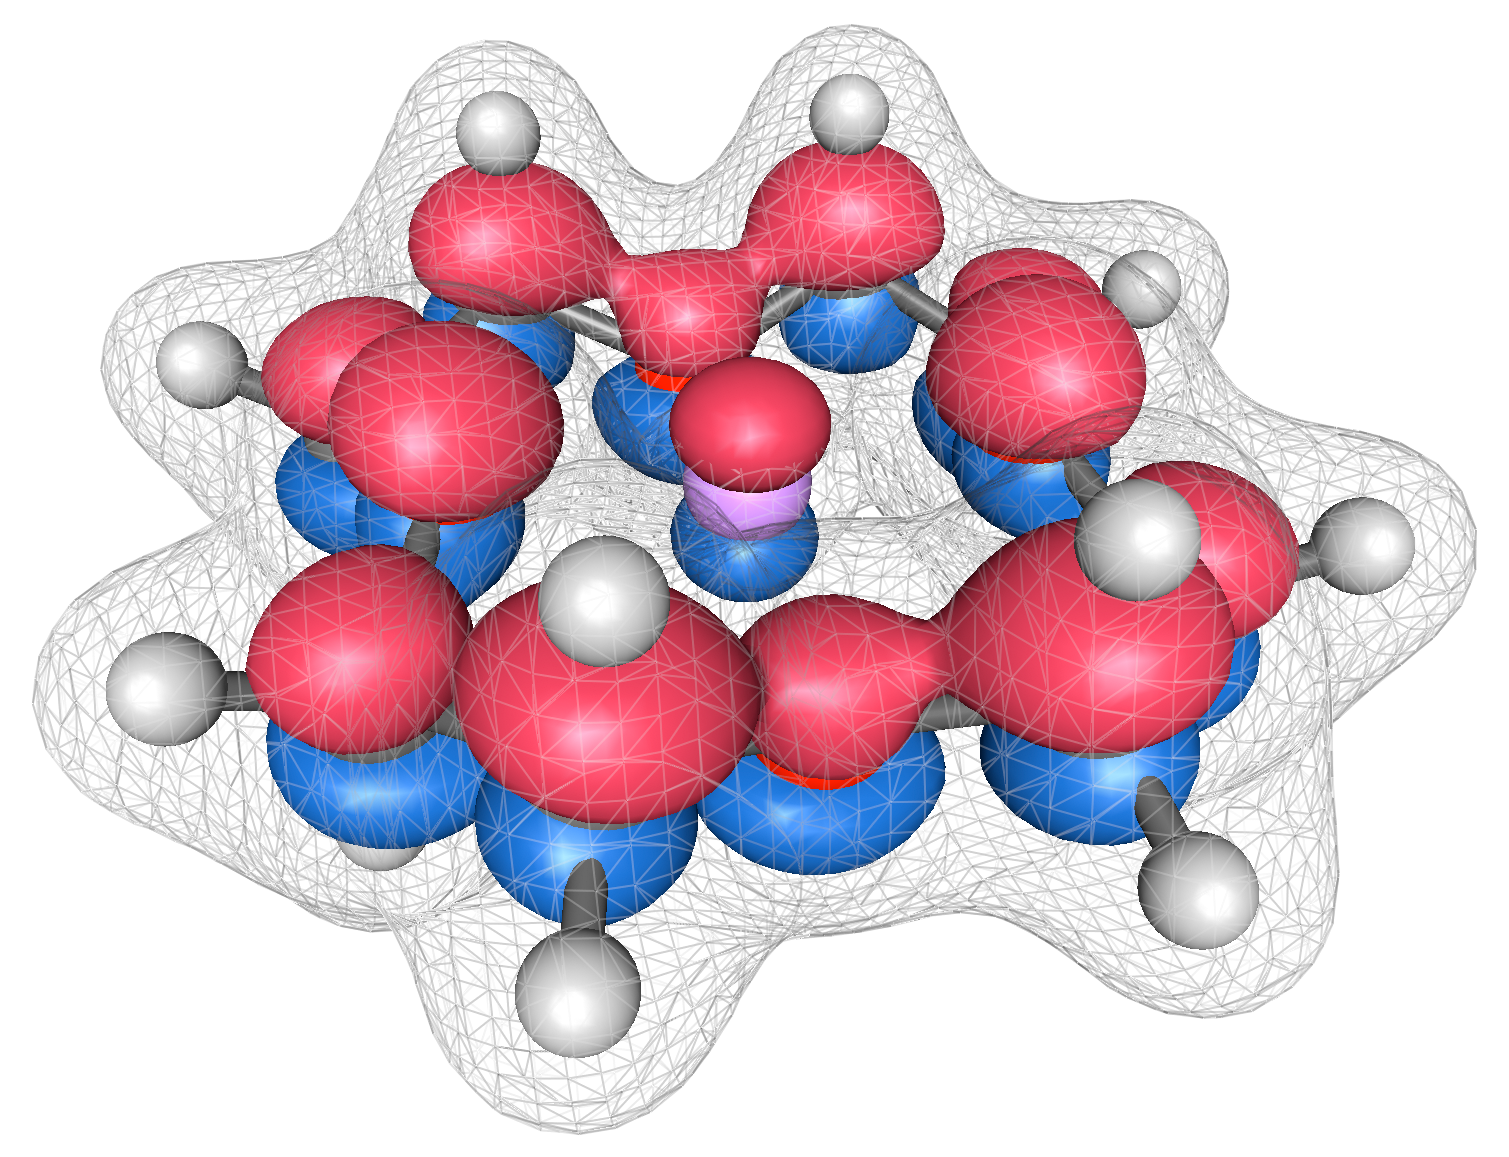
\includegraphics[scale=0.25]{figures/Crown.png}
\end{center}

\vfill
\myline\\
\begin{center}
{\large v2.7 (2015) Andrew Gilbert}
\end{center}
\myline\\

\newpage


%----------------------------------------------------------------------%
\section{Introduction}
%----------------------------------------------------------------------%

\iqmol{} is an open-source molecular editor and visualization package that runs
under Windows, Mac OS X and Linux.  It can read a variety of chemical file
formats including xyz, cml, pdb, mol, fchk, cube data and \qchem{}
input/output.  It also includes a free-form molecular builder that allows
arbitrary molecular structures to be created.  These structures can be
optimized using molecular mechanics force fields and symmetrized to ensure the
strucuture has the correct point group symmetry.  A library of molecules and
functional groups also exists and these can be used to facilitate building
molecules. \\

\iqmol{} is capable of displaying a variety of molecular properties including
atomic charges, dipole moments and normal modes.  Several surface types can be
displayed including molecular orbitals, (spin) densities and van der Waals
surfaces, and these can be colored according to an arbitrary scalar field such
as the electrostatic potential.  Animations are also available for vibrational
frequencies and reaction and optimization pathways. \\

\iqmol{} can operate as a stand-alone package, but has also been written to
work seamlessly with the \qchem{} computational chemistry package.  A
comprehensive input file generator, the \qchem{} User Interface (QUI), provides
access to most of the available options in \qchem{}, and these options are
presented in an intuitive, hierarchical fashion.   The generated input files can
be submitted to either local or remote servers that have the \qchem{} software
installed.  In particular, a publicly accessable server is available that
allows small (limited to approximately 5 mins) quantum chemistry calculations to
be run without having to purchase and install \qchem{}.



\subsection{Installation}

The latest version of \iqmol{} can be downloaded from the website:
\begin{center}
\url{http://iqmol.org/downloads.html}
\end{center}

For Mac (OS X) a disk image file is provided.  Simply double click the disk
image after downloading and copy the application to the Applications directory,
or any other desired location. \\

For Windows and Linux an installer is provided that will guide you through the
installation process and will also create a shortcut on your desktop.


\newpage
\subsection{Overview}

\begin{center}
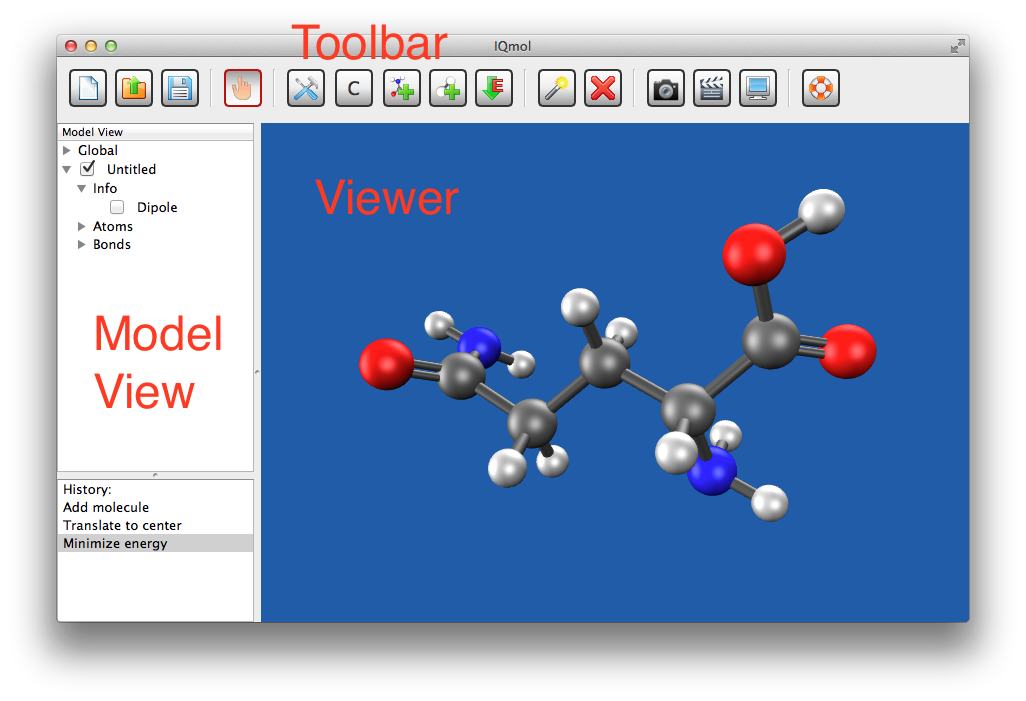
\includegraphics[scale=0.40]{figures/Viewer.png}
\end{center}

The main \iqmol{} window is shown above and comprises the following main parts:
\begin{itemize}
\item The {\bf Viewer} is the main part of the window and is where you can
      view and interact with your molecule.
\item The {\bf Toolbar} at the top provides access to common commands and allows selection
      between different viewer modes including manipulation 
      
\includegraphics[scale=0.40]{figures/ManipulateButton.png}, selection 
      
\includegraphics[scale=0.40]{figures/SelectButton.png} and building.
      
\includegraphics[scale=0.40]{figures/BuildButton.png}
\item The {\bf Model View} panel provides a hierarchical view of the data that
      are available for the molecule.
\item The {\bf History} panel in the lower left shows a list of the most recent
      actions than can be undone, either by clicking on them or by using the
      Edit $\blacktriangleright$ Undo menu option. 
\end{itemize}

The Model View (MV) provides control over what objects are displayed in the Viewer
and also allows access to configuration options for these objects.  Visibility is
controlled by the associated checkbox.  Unchecking a checkbox causes the item
and all its children to become hidden.  If an item does not have a checkbox,
for example a bond, then its visibility can only be controlled by items higher
in the hierarchy.  \\

The appearance of many objects can be configured by double-clicking the item in
the MV.  For example, double-clicking the molecule name brings up the Configure
Molecule dialog:
\begin{center}
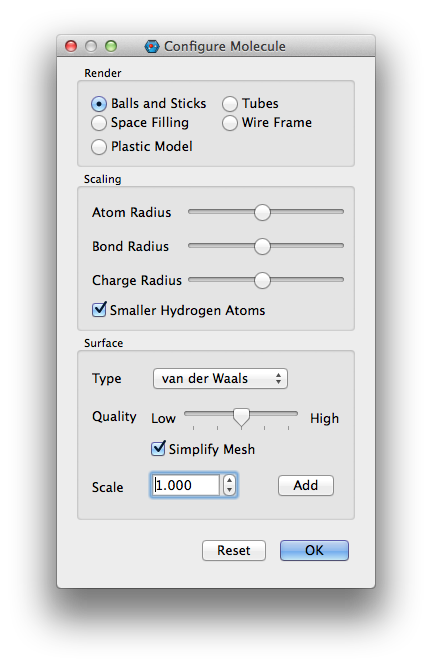
\includegraphics[scale=0.40]{figures/MoleculeConfigurator.png}
\end{center}
Along with selecting different rendering options (see below), this
dialog also allows several types of surface plot to be generated including van
der Waals, promolecule and superposition of ionic densities (SID). \\
\begin{center}
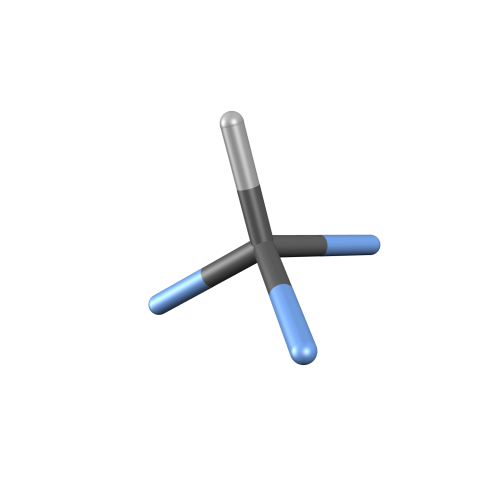
\includegraphics[scale=0.25]{figures/CHF3-tubes.png}\hspace{-15mm}~
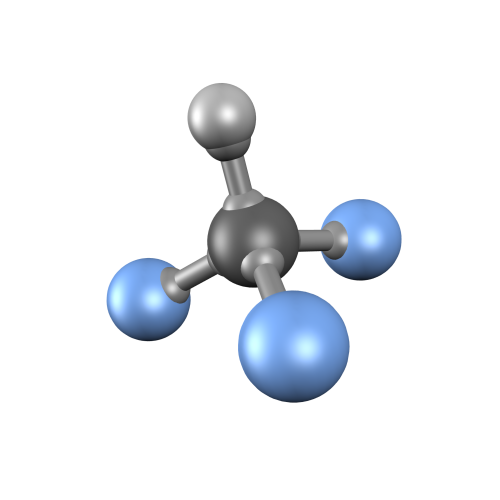
\includegraphics[scale=0.25]{figures/CHF3-moly.png}\hspace{-15mm}~
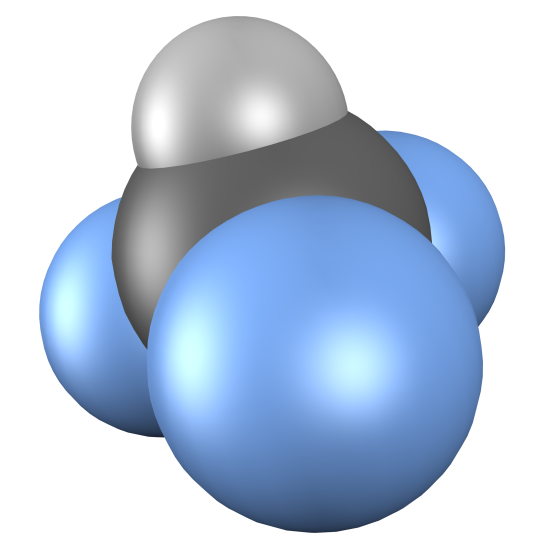
\includegraphics[scale=0.25]{figures/CHF3-space.png}
\end{center}
Note that several molecules can be viewed concurrently in the same Viewer
and each of these can be configured separately.  





%----------------------------------------------------------------------%
\newpage
\section{Building Molecules}
%----------------------------------------------------------------------%


\subsection{Adding Atoms and Fragments}

By default, \iqmol{} opens in build mode.  This is indicated by a red border
around the 
\includegraphics[scale=0.40]{figures/BuildButton.png} button in the
Toolbar.   The default build atom is indicated by the

\includegraphics[scale=0.40]{figures/BuildAtomButton.png} button and can be changed
by clicking on this button.  A pop-up periodic table will appear from which the
desired element type can be selected. \\

Clicking in the empty Viewer window will create an atom of the current build
element. Additional atoms can be added by clicking on an existing atom and
dragging the mouse.  This creates a new atom bonded to the first.  To create a
disconnected atom, hold down the \emph{alt} modifier key when clicking in the
Viewer window.  (Note that some Linux window managers use the \emph{alt} modifier
for other purposes.  This behavior can be changed using System Settings 
$\blacktriangleright$ Keyboard $\blacktriangleright$ Short-cuts menu). \\

Bond orders can be increased by clicking and dragging between two existing
atoms.  If no bond exists between the two atoms,  one is created.  Otherwise
the bond order is increased.  To decrease the bond order, the bond must first
be deleted and a new bond created.
\begin{center}
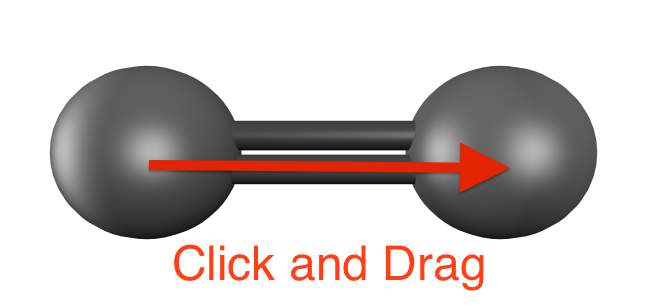
\includegraphics[scale=0.25]{figures/Cdouble.png}
\end{center}


Functional groups can be added by clicking the

\includegraphics[scale=0.40]{figures/BuildFragButton.png} button, ensuring the
Functional Group radio button is clicked and selecting the desired group from
the menu.  Groups are added in the same way as atoms, \emph{i.e.} clicking and
dragging from an existing atom.  The empty valence is indicated by the yellow
bond and shows where the group will be connected.
\begin{center}
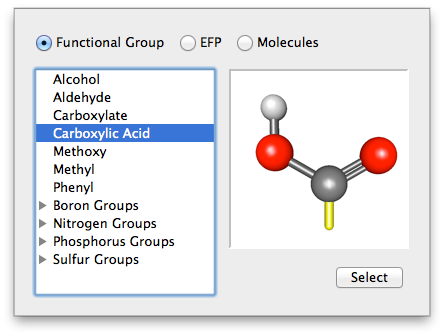
\includegraphics[scale=0.5]{figures/FunctionalGroup.png}
\end{center}

Entire molecules can be added to your system by clicking the

\includegraphics[scale=0.40]{figures/BuildFragButton.png} button, ensuring the
Molecules radio button is clicked and selecting the desired molecule from the
menu.  Unlike the other build modes, clicking anywhere in the viewer window
will add the selected molecule, (no mouse modifier is required).  This allows
several molecules of the same type to be added quickly, (\emph{e.g.} for
solvation), but changes the usual mouse behavior.  If you accidentally add 
too many molecules, use the Edit $\blacktriangleright$ Undo menu option. \\
%\begin{center}
%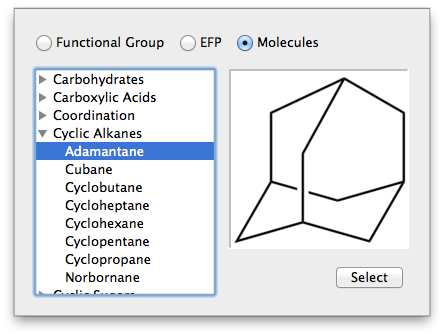
\includegraphics[scale=0.5]{figures/BuildMol.png}
%\end{center}

Once the backbone of the molecule has been draw the Add Hydrogens button

\includegraphics[scale=0.40]{figures/AddHydrogensButton.png} can be clicked to add
hydrogen atoms to any unfilled valencies.



\subsection{Cleaning Up Geometries}

The builder in \iqmol{} is free-form, so your initial structure may look a bit
wonky.  To improve the geometry, click the

\includegraphics[scale=0.40]{figures/MinimizeEnergyButton.png} button.  This
optimizes the geometry using a molecular mechanics (MM) force field.   The default
force field is the Universal Force Field (UFF) which has the advantage of being
defined for most of the periodic table.  However, the UFF does not perform well
for systems with hydrogen bonds and in these cases it is recommended that the
force field be changed by going to the Build $\blacktriangleright$ Select Force Field menu
option.

\begin{center}
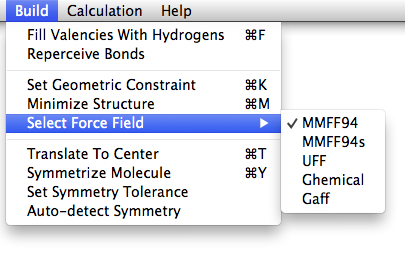
\includegraphics[scale=0.5]{figures/ForceFieldMenu.png}
\end{center}

If your molecule has symmetry, the MM optimization is unlikely to find a
structure with the desired symmetry.  If this is the case, a nearly symmetric
structure can be symmetrized using the Build $\blacktriangleright$ Symmetrize Molecule
menu option.  Finding very high symmetry may require relaxing the tolerance
using the Build $\blacktriangleright$ Set Symmetry Tolerance menu option.

\subsection{Specifying Geometric Parameters}

Specific values for geometric parameters can be set by first selecting the
atoms involved and using the Build $\blacktriangleright$ Set Geometric Constraint menu
option.  A dialog will appear that allows the parameter to be either set,
constrained or scanned.  Constrained parameters apply to any subsequent MM
optimization and are also passed through to the \qchem{} input file, if a
optimization job is requested.  Scan options are also passed through to
\qchem{} for scan jobs. \\

\begin{center}
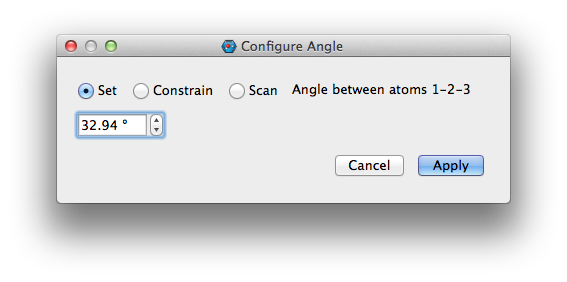
\includegraphics[scale=0.5]{figures/ConstraintDialog.png}
\end{center}

The type of constraint depends on the number of atoms selected:
\begin{enumerate}
\item Fixed atom position
\item Inter-atomic distance (or select a single bond)
\item Bond angle
\item Torsion (dihedral) angle
\end{enumerate}

Active constraints are visible in the Viewer and can be deactivated by clicking
the adjacent checkbox in the MV.


\subsection{Manipulating and selecting molecules}

Select mode is activated by clicking the 

\includegraphics[scale=0.40]{figures/SelectButton.png} button and implements 
the following mouse functions:

\begin{itemize}
\item {\bf Left click:} Adds atom or bond to selection. 
\item {\bf Click and drag:} Creates a selection rectangle, all atoms and bonds
           within the selection rectangle are added to the selection. 
\item {\bf Right click:}  Removes atom or bond from selection.
\end{itemize}


Manipulate mode is activated by clicking the 

\includegraphics[scale=0.40]{figures/ManipulateButton.png} button and implements 
the following mouse functions:

\begin{itemize}
\item {\bf Left click and drag:} Rotate the view of the molecule.  
\item {\bf Middle click and drag:} Zoom in and out.  
\item {\bf Right click and drag:} Translate the view of the molecule.
\end{itemize}

It is also possible to manipulate part of the molecule independently from the
rest.  To do this, make a selection and press and hold the \emph{ctrl} modifier
(\emph{command} key on Mac).  The mouse movements will affect only the 
selected atoms as follows:

\begin{itemize}
\item {\bf Left click and drag:} Rotate the selected atoms about their center. 
\item {\bf Right click and drag:} Translate the selected atoms.  
\end{itemize}

If a single bond is selected, then the mouse movements have the following effects
\begin{itemize}
\item {\bf Left click and drag:} Rotate around the axis of the bond.
\item {\bf Right click and drag:} Change the length of the bond.
\end{itemize}








%----------------------------------------------------------------------%
\newpage
\section{Running \qchem{} Calculations}
%----------------------------------------------------------------------%

\subsection{The QUI}

\iqmol{} has a built-in input file generator for \qchem{} calculations, the
QUI, that can be accessed via the Calculation $\blacktriangleright$ Q-Chem
Setup menu.  
\begin{center}
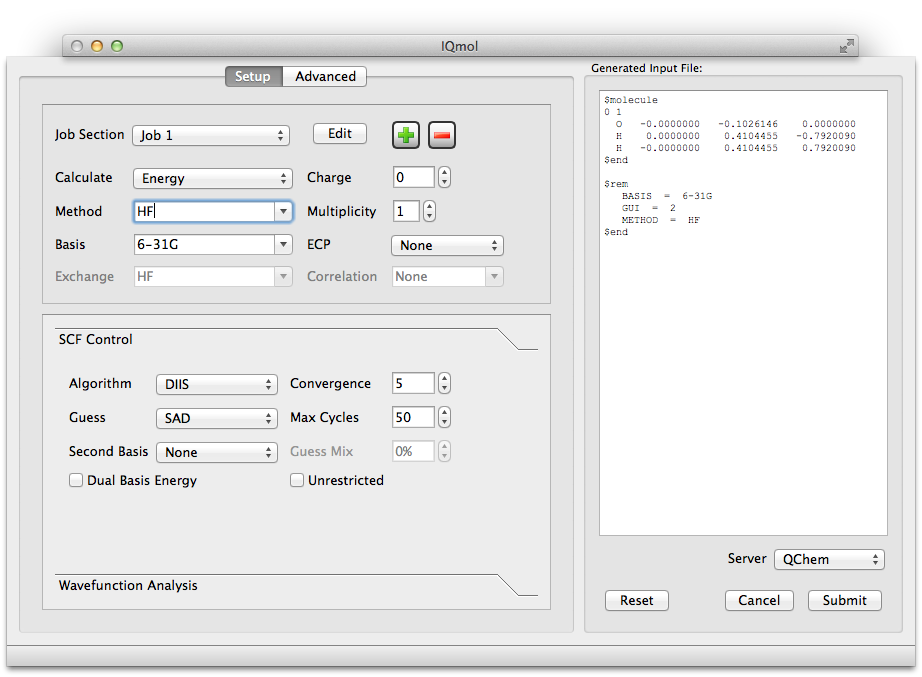
\includegraphics[scale=0.4]{figures/QUI.png}
\end{center}
The left hand side of the QUI dialog contains controls for setting up the
calculation.  These are presented in a hierarchical fashion so that most
commonly used options are presented in the top part of the panel, with other
relevant options appearing in the lower section depending on what type of job
is selected.  More advanced options can be accessed via the Advanced tab.  The
generated input file is echoed in the panel on the right hand side of the QUI.\\

Clicking the Submit button will start the job running on the selected server.
Once the job has completed you will be prompted to copy the results (for remote
servers) before they are automatically loaded into \iqmol{}.  The

\includegraphics[scale=0.6]{figures/Favourites.png} icon appears next to the
molecule name in the MV when the molecule has been updated with the
results of a calculation.

\subsection{The Job Monitor}

Submitted jobs can be monitored via the Calculation $\blacktriangleright$ Job
Monitor menu option.  This brings up the Job Monitor dialog that provides
information on the progress of jobs.  Right-clicking a row in the Job
Monitor brings up a context menu which allows running jobs to be killed or
queried, and finished jobs to be opened.
\begin{center}
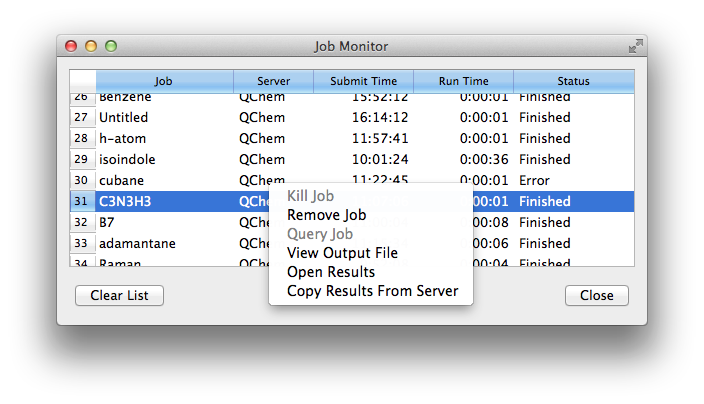
\includegraphics[scale=0.5]{figures/JobMonitor.png} \\
\end{center}
If a job has the Error status, hovering the mouse over the status will 
show the error message.  Alternatively, double clicking the job will open
the output file, if available.


\subsection{Configuring Servers}

By default \iqmol{} is configured to submit jobs to the HTTP \qchem{} server in
Pleasanton, California.  This is a publicly available server than can be used
by anyone wishing to run test calculations before purchasing the \qchem{}
software.  Jobs submitted to this server can access the full suite of
electronic structure methods available in \qchem{}, but are time-limited to 5
minutes. \\

Additional servers can be configured to access other computers that have the
\qchem{} software installed.  These computers can be either local servers
(\emph{i.e.}  the same machine as the one running \iqmol{}) or remote servers
that can be connected  via SSH.  To add an additional server, go to the
Calculation $\blacktriangleright$ Edit Servers menu option and click the

\includegraphics[scale=0.40]{figures/PlusButton.png} button.  
\begin{center}
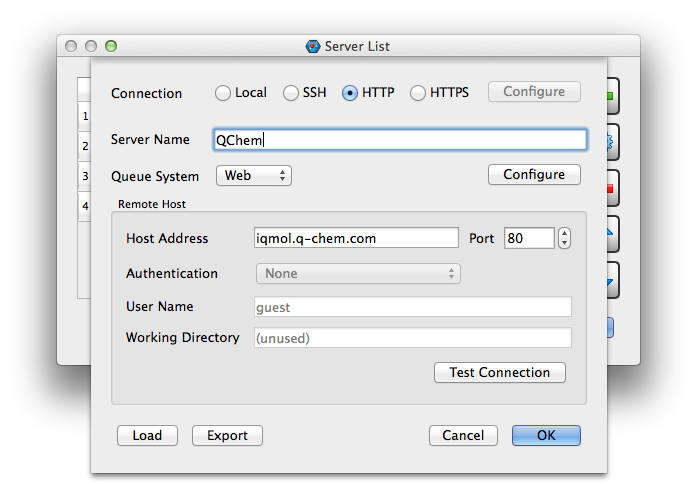
\includegraphics[scale=0.5]{figures/ServerDialog.png}
\end{center}

The information required to configure a server depends on its type, but default
options exist for each case.  The following indicates the minimum that should
be considered:

\begin{itemize}
\item {\bf Local:} Set the Queue System to `Basic'
      unless you know you are running queuing software on the machine.
      Be sure the {\tt QC} and {\tt QCSCRATCH} variables are set to their correct
	  values in the Run File Template, which is accessed by clicking the Configure
      button.
\item {\bf SSH:} The hostname and account on the target machine will 
      be required in order to connect via SSH.  Set the Authentication combo-box to
      `Password Prompt' unless you have set up an alternative authentication protocol.
	  Depending on how the target host has been set up, the Run File Template
	  may require some editing to get it to work, but this will differ from
      machine to machine.
\item {\bf HTTP:} The default options should be suitable.
\end{itemize}


%----------------------------------------------------------------------%
\newpage
\section{Analyzing Results}
%----------------------------------------------------------------------%

\subsection{Plotting Molecular Orbitals}
Plotting molecular orbitals (MO) requires a formatted checkpoint file (.fchk)
which is generated by default when running \qchem{} calculations using \iqmol{}
(GUI rem variable should be set to 2).  After opening the file, a MO Surfaces
item will be available in the MV, double-clicking this brings up the Add Surface
dialog:
\begin{center}
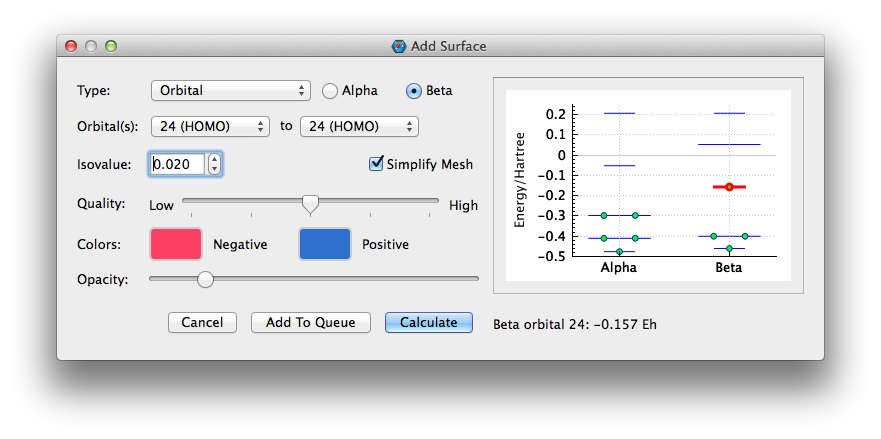
\includegraphics[scale=0.5]{figures/MolecularOrbitalsConfigurator.png} \\
\end{center}
The dialog allows both MOs and densities to be computed, and several surfaces
can be computed at the same time (this is more efficient as the shell data
only needs to be computed once).  The quality, colors and opacity of the
surfaces can be be set in the dialog, and changes to these settings are saved
to the preferences as default values for future surfaces.  Once computed, the
individual surfaces appear as sub-items in the MV and these can be further
configured by double-clicking the items in the MV.  \\

The Add Surface dialog also contains an interactive energy level diagram.  The
vertical scale can be zoomed in and out using the scroll wheel (or equivalent)
on the mouse.  The scale can also be translated by a left click-and-drag.
Individual orbitals can be selected with a left-click and this will cause the
energy of the selected orbital to appear below the diagram. \\

The grid data generated for each surface is stored internally so that
subsequent calculations of the same surface (with different isovalues, for
example) are much faster.  To see what grid data is being stored, right-click
on the MO Surfaces item in the MV to bring up the context menu.  Selecting the
Show Grid Info menu brings up the Grid Information dialog:
\begin{center}
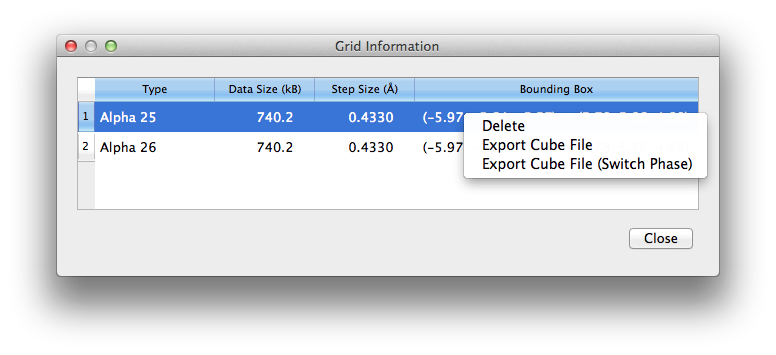
\includegraphics[scale=0.5]{figures/GridInfo.png} \\
\end{center}
From this dialog it is possible to export cube files containing the grid data.
Right-clicking on the desired grid brings up a context menu with the option
Export Cube File option.  The Switch Phase option swaps the sign of the data
and may be useful when comparing two systems where the (arbitrary) phases
differ.  Cube files can be saved for future plotting to avoid having to
recompute the data, or for reading into another plotting package. \\


\subsection{Visualizing Cube File Data}

Cube files contain volumetric data such as electron densities, molecular
orbitals or electrostatic potentials (ESP).  Because the data has been
pre-computed, generating surfaces using them is very quick.  After opening a
cube file, a Cube Data item will appear in the MV, double-clicking this item
brings up the Add Surface dialog:  
\begin{center}
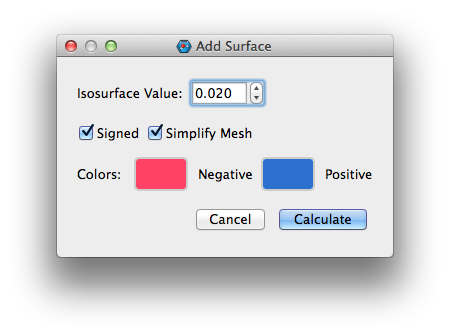
\includegraphics[scale=0.5]{figures/AddSurface.png} \\
\end{center}
The Signed checkbox causes two isosurfaces to be generated corresponding to
$\pm$ the specified isovalue, and this should be checked for data such as MOs
and spin densities.\\

Cube file data can also be used to color a surface and this will require either
two cube files (one containing the surface data and the second containing the
property used to color the surface) or a cube file and a checkpoint file.  In
either case two files need to be loaded into the one molecule.  To do this,
ensure the files are in the same directory and have the same base name
(everything up to the first `.').  For example, the directory might be named
`Benzene' and contain the files `Benzene.esp.cube' and `Benzene.fchk'.  The
File $\blacktriangleright$ Open Dir menu option can be used to open the
directory and both the cube and fchk files will be loaded into the Benzene
molecule in the MV.  \\

After creating a surface, as detailed above, double-clicking the surface item will
cause the Configure Surface dialog to appear:
\begin{center}
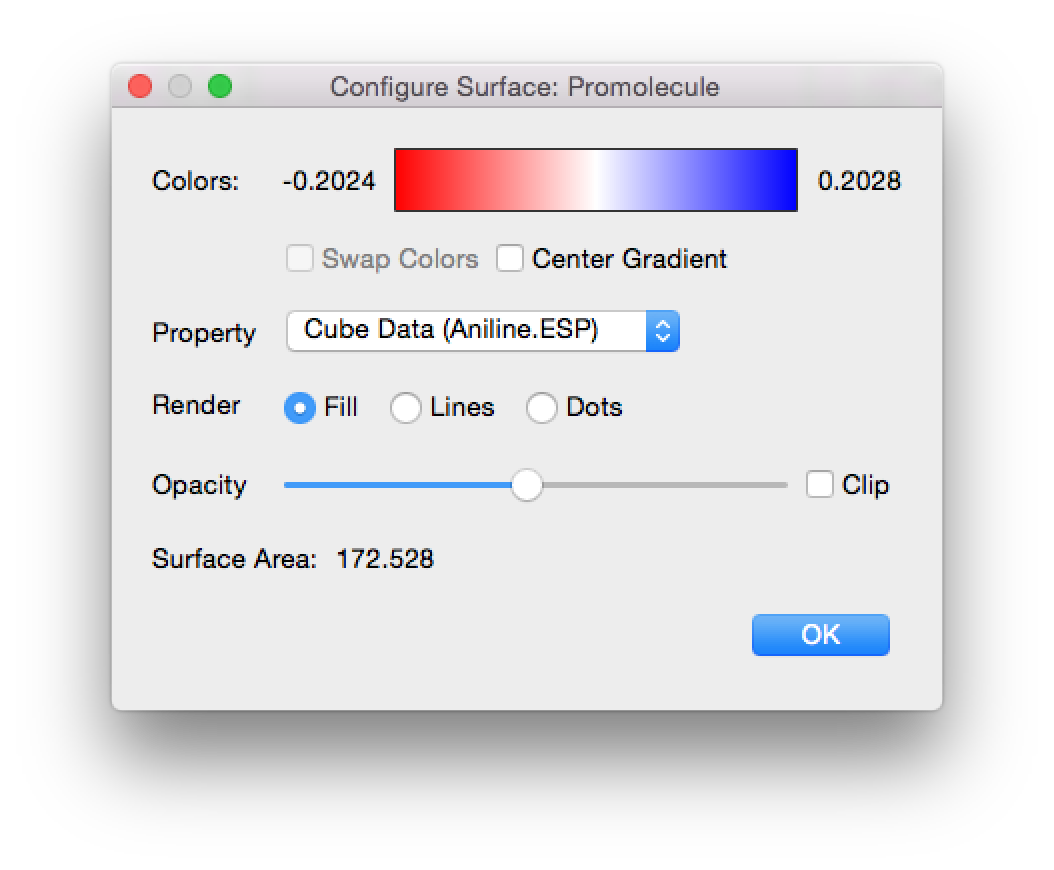
\includegraphics[scale=0.5]{figures/SurfaceConfigurator.png} \\
\end{center}
The Property combo-box will have the cube data as one of the options, and selecting
this will cause the surface to be colored according to the data in the cube file.
The gradient colors can be altered by clicking inside the gradient box.
\begin{figure}[hb]
\begin{center}
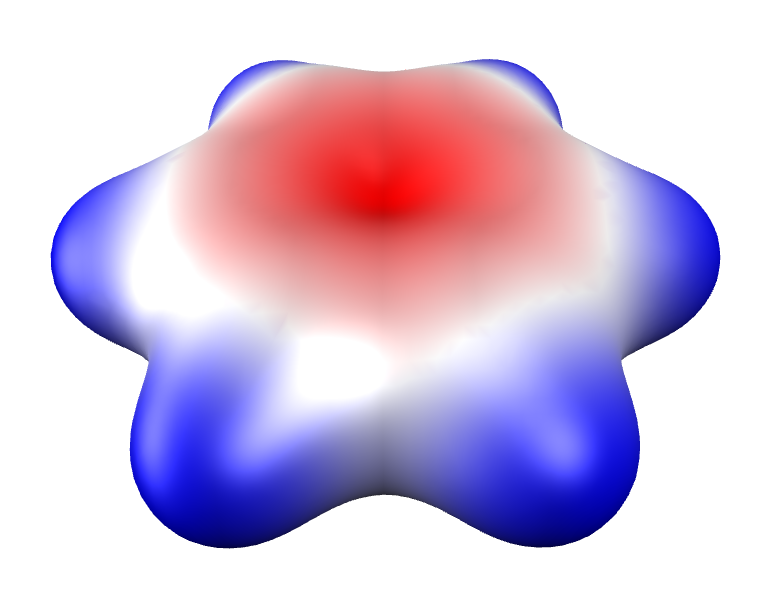
\includegraphics[scale=0.3]{figures/Benzene.png} \\
\end{center}
\caption{Electron density plot of benzene colored according to the electrostatic potential}
\end{figure}


\newpage
\subsection{Potential Energy Surfaces}

Several job types provide slices through the potential energy surface (PES).
These include geometry optimizations, PES scans, reaction pathways  and
transition state searches.  On opening a \qchem{} output file containing one of
these job types a Geometries item appears in the MV and can be double-clicked
to bring up the Geometries dialog.
\begin{center}
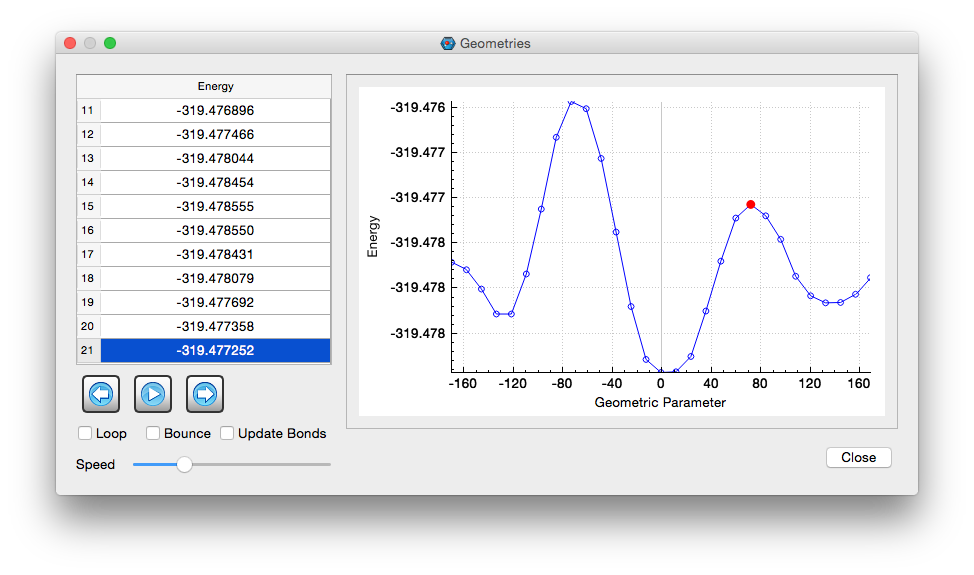
\includegraphics[scale=0.40]{figures/PesScan.png} \\
\end{center}
The pathway can be animated in the viewer using the play button and individual
frames can be selected from the table or on the plot and the viewer will be
updated with the corresponding structure.\\

Pathways can also be read in from an XYZ file.  The format for this is simply a
concatenation of regular XYZ files:
{\footnotesize
\begin{verbatim}
5
-291.77177
Si  0.71979   -0.08082   -0.76577  
H   0.73262   -1.27801    0.22990   
H   1.10451    0.93673    0.34825   
H  -1.32980    0.23894   -0.28240  
H  -1.22713    0.18317    0.47002   
5
-291.76961
Si  0.67218   -0.07483   -0.72935  
H   0.73053   -1.29428    0.22634   
H   1.10815    0.95270    0.34714   
H  -1.29502    0.23567   -0.33016  
H  -1.19409    0.17584    0.49156 
....
\end{verbatim}
}
The first line gives the number of atoms, the second (comment) line must have
the corresponding energy and then the following lines have the xyz coordinates
of each atom in the system.  This pattern repeats for as many frames as you have
available.



\newpage
\subsection{Vibrational Frequencies}

Vibrational frequencies can be read in from a \qchem{} output file and appear
as a Frequencies item in the MV.  Normal mode vectors can be visualized by
selecting the associated frequency item in the MV.
\begin{center}
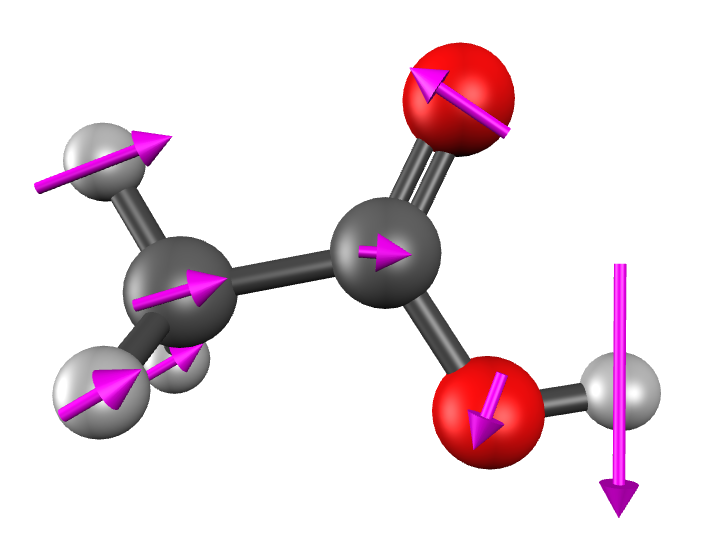
\includegraphics[scale=0.25]{figures/VibMode.png} \\
\end{center}
Double-clicking a frequency in the MV will cause the molecule to vibrate
according to the selected mode.  Double-clicking the Frequencies item will
bring up the Vibrational Frequencies dialog:
\begin{center}
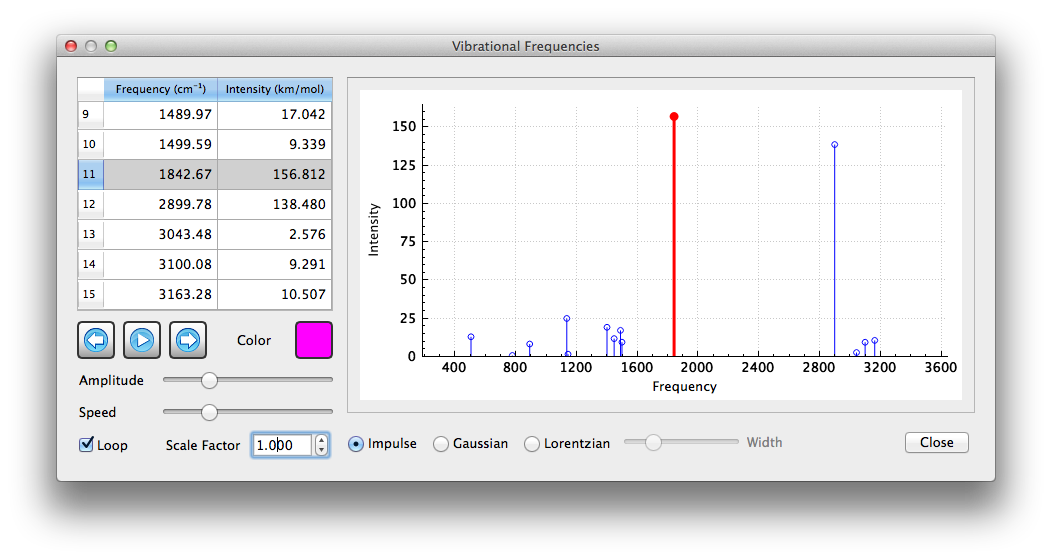
\includegraphics[scale=0.40]{figures/Frequencies.png} \\
\end{center}
This dialog contains an impulse spectrum showing the positions and relative
intensities of the frequencies.  Individual modes can be selected on the
spectrum by clicking the hollow circles and this will also update the Viewer
window with the selected mode.  The impulses can be broadened using either
Gaussians or Lorentzians to give a more realistic looking spectrum. \\

The horizontal scale of the spectrum can be zoomed (using the scroll wheel on
the mouse) and translated (left-click and drag) to give greater detail.


\newpage
\subsection{NMR Spectra}

NMR shieldings and chemical shifts can be visualized using \iqmol{}.  A 
\qchem{} calculation (JOB\_TYPE = NMR) must first be run and the output
file opened.  Shielding constants can be displayed as atom labels in the
viewer by selecting the Display $\blacktriangleright$ Atom Labels  
$\blacktriangleright$ NMR option.
\begin{center}
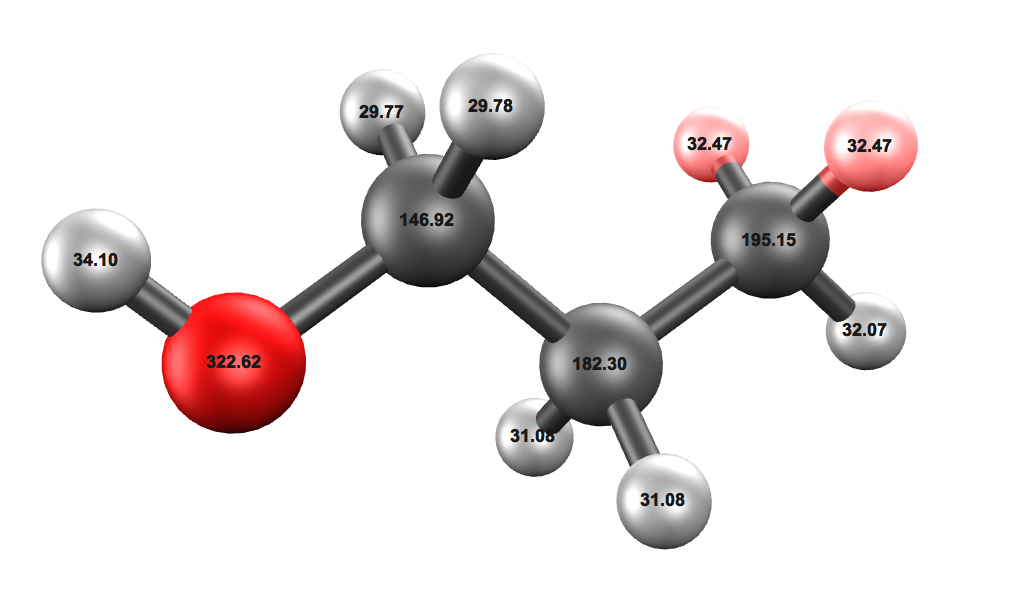
\includegraphics[scale=0.25]{figures/NmrDisplay.png} \\
\end{center}
An NMR item will appear on in the MV and double-clicking this brings up the NMR
Spectrum dialog.
\begin{center}
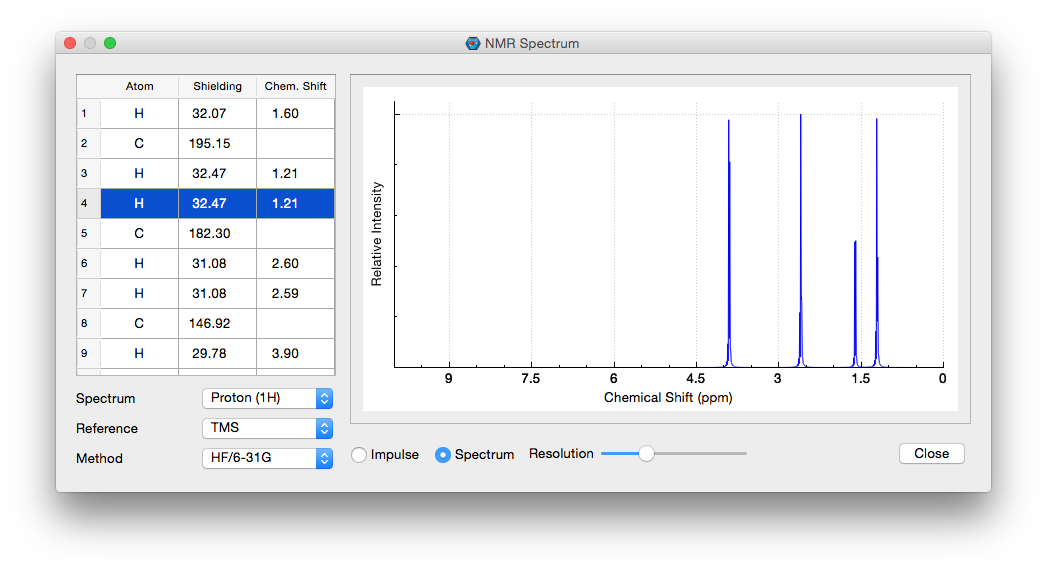
\includegraphics[scale=0.40]{figures/NmrConfigurator.png} \\
\end{center}
Various spectrum types can be displayed ($^1$H, $^{13}$C etc) and if 
a reference is available (e.g. TMS) for the given level of theory, 
chemical shifts can also be displayed.  Selecting rows in the table
will also highlight the corresponding atoms in the viewer for easy
identification.  If impulses are plotted, then these can also be selected
to identify which atoms are responsible for the selected signal.




%----------------------------------------------------------------------%
\end{document}
%----------------------------------------------------------------------%

\subsection{Reaction Pathways}
xyz files

\subsection{ESP}

\subsection{Orbital Animations}
requires cube files

\subsection{Making Movies}

\subsection{Configuration}
The Global item in the MV is always available and allows 

Preferences
The default MM force field c
appearance
Global


